\chapter{%
Problemas de Sturm-Liouville
}




\section{Problemas físicos que llevan a problemas de Sturm-Liouville}
{Ecuación del Calor}

\emph{Bibliografía}
R. Kent Nagle, Edward B. Saff \& Arthur David Snider. Ecuaciones diferenciales y problemas con valores en la frontera


Recordemos la ecuación diferencial del Calor \emph{Acordate repasar deducción}

\[ \frac{\partial c\rho u}{\partial t}-\operatorname{div}( k \nabla u)=S \]

con:

\begin{itemize}
\item $u$ temperatura del medio
 \item $c$  calor específico
 \item $\rho$ densidad
 \item $k$ coeficiente conductividad térmica
 \item $S$ fuente externa de calor
\end{itemize}

$c, \rho, k, S$ son funciones del tiempo $t$ y el espacio $(x,y,z)$. 



{Ley Enfriamiento de Newton}


En algunos problemas la fuente externa $S$  además de contener términos $h(x,y,y,t)$ que dependen de la posición y el tiempo contiene otros que dependen de  la temperatura $u$. 


Por ejemplo en la \emph{Ley Enfriamiento de Newton} el calor que ingresa a un cuerpo  es proporcional a la diferencia de temperatura entre el cuerpo y el medio circundante. 


 La ecuación se transforma

 \begin{empheq}[box=\tcbhighmath]{equation}\label{eq:calor+newton}
 \frac{\partial c\rho u}{\partial t}- \dive k \nabla u - q u=h.
\end{empheq}

También $q$ podría ser función de $t$ y $(x,y,z)$.



{Ecuación del calor uni-dimensional}

Para mayor simplicidad nos restringiremos al caso de un alambre recto y tan delgado que la asumimos uni-dimensional. La única variable espacial es $x\in [a,b]$ y $t>0$.

{\small
 \begin{empheq}[box=\tcbhighmath]{equation}\label{eq:calor-uni} 
 \quad c(x) \rho(x) \frac{\partial u}{\partial t}(x, t)=\frac{\partial}{\partial x}\left[k(x) \frac{\partial u}{\partial x}(x, t)\right]+q(x) u(x, t)+h(x, t).
 \end{empheq}
 }
 
 


{Condiciones de contorno e iniciales}

\textbf{Condiciones de contorno: en $x=a$ o $x=b$}

\begin{description}
 \item[ Extremos fijos (Dirichlet)] $u=0$
 \item[Alambre aislado (Neuman)]   $\partial u / \partial x=0$
 \item[Condiciones mixtas] $\partial u / \partial x+c u=0$.
\end{description}

Para generalizar la situación, supondremos

\begin{empheq}[box=\tcbhighmath]{equation}\label{eq:cond_cont}
\left\{\begin{array}{cc}
 a_{1} u(a, t)+a_{2} \frac{\partial u}{\partial x}(a, t)&=0\\ b_{1} u(b, t)+b_{2} \frac{\partial u}{\partial x}(b, t)&=0
\end{array}
\right.\end{empheq}
  
\textbf{Condiciones iniciales}
$$u(x,0)=f(x)$$
   
 


{Problema}

Para simplificar nuestro problema supondremos que $h(x, t) \equiv 0$. 
Vamos a estudiar el siguiente problema de contorno y valores iniciales.



{\small
\begin{empheq}[box=\tcbhighmath]{equation}\label{eq:calor_main}  
\left\{
        \begin{array}{ll}
            r(x) \frac{\partial u}{\partial t}(x, t)=\frac{\partial}{\partial x}\left[p(x) \frac{\partial u}{\partial x}(x, t)\right]+q(x) u(x, t) &   a<x<b,  t>0,\\
            & \\
             a_{1} u(a, t)+a_{2} \frac{\partial u}{\partial x}(a, t)=0 &\  t>0,\\
             &\\
              b_{1} u(b, t)+b_{2} \frac{\partial u}{\partial x}(b, t)=0 & t>0,\\
              &\\
            u(x, 0)=f(x)&   a<x<b.
        \end{array}
\right. \notag
\end{empheq}
}

donde $r(x)=c(x) \rho(x)$ y $p(x)=k(x)$.

   
 


{Problemas Sturm-Liouville}

\begin{ejercicio}{}[Separación Variables]
 
Supongamos $u(x, t)=y(x) T(t)$ resuelve la ecuación,  reemplazando en la ecuación principal demostrar  que existe $\lambda\in\rr$ (es un número por determinar)
\[
 \left\{
        \begin{array}{ll}
        \frac{d}{d x}\left[p(x) \frac{d y}{d x}\right]+q(x) y+\lambda r(x) y=0 & a<x<b,\\
        a_{1} y(a)+a_{2} y^{\prime}(a)=0, &\\
        b_{1} y(b)+b_{2} y^{\prime}(b)=0 & \\
        \end{array}
 \right.
 \]
\end{ejercicio}

Este sistema se llama  un \emph{problema de Sturm-Liouville} con valores en la frontera. 

Excluimos las condiciones triviales en la frontera, donde $a_{1}=a_{2}=0$ o $b_{1}=b_{2}=0$. 



 
 

\subsection{Clasificación}
{Clasificación problemas Sturm-Liouville}
\begin{definicion}
 Cuando:
 \begin{itemize}
  \item  $p(x), q(x)$ y $r(x)$ son continuas en $[a, b]$, 
  \item $p'$ derivable en $(a,b)$,
  \item $p(x)>0$ y $r(x)>0$ en $[a, b]$, 
 \end{itemize}
decimos que tenemos un  \emph{ problema regular de Sturm-Liouville}.


Decimos que la ecuación es \emph{singular} si:
 \begin{itemize}
  \item $p$ se anula en $a$ o  $ b$,
  \item si $p(x), q(x)$ o $r(x)$ no están acotadas cuando $x$ tiende a $a$ o a $b$,
  \item cuando el intervalo $(a, b)$ no está acotado. 
 \end{itemize}



  
\end{definicion}


 
 

{Clasificación problemas Sturm-Liouville}


\textbf{Ejemplo (problema singular):} Problema contorno para la Ecuación de Bessel en $[0,b]$

\[
 \left\{
        \begin{array}{l}
         \frac{d}{d x}\left[x \frac{d y}{d x}\right]+\lambda x y=0, \quad 0<x<b\\
         \lim _{x \rightarrow 0^{+}} y(x)\hbox{ y }\lim _{x \rightarrow 0^{+}} y^{\prime}(x) \hbox{ existen y son finitos},\\ 
         y(b)=0 .\\         
        \end{array}
 \right.
\]

Este problema surge al estudiar el flujo de calor en un cilindro. En este caso, $p(x)=r(x)=x$, que se anula en $x=0$. 

 

\section{Problemas de contorno} 
 
\subsection{Clasificación condiciones de contorno}
 
{Problemas contorno ecuaciones lineales ordinarias de segundo orden}

Supongamos el problema de contorno

\[
 \left\{
        \begin{array}{l}
            y^{\prime \prime}+p(x) y^{\prime}+q(x) y=f(x), \quad 0<x<b\\
            a_{11} y(a)+a_{12} y^{\prime}(a)+b_{11} y(b)+b_{12} y^{\prime}(b)=c_{1}\\
            a_{21} y(a)+a_{22} y^{\prime}(a)+b_{21} y(b)+b_{22} y^{\prime}(b)=c_{2}\\ 
         \end{array}
 \right.
\]

Estas son condiciones de contorno lineales. Cuando $c_{1}=c_{2}=0$, decimos que las condiciones de contorno  son \emph{homogéneas}; en caso contrario, son \emph{no homogéneas}.



{Clasificación condiciones de contorno}
Ciertas condiciones en la frontera aparecen con frecuencia en las aplicaciones; estas condiciones son

\begin{description}
 \item[Separadas:]<+->
 \[\begin{split}
    a_{1} y(a)+a_{2} y^{\prime}(a)&=c_{1},\\
    b_{1} y(b)+b_{2} y^{\prime}(b)&=c_{2}
   \end{split}
\]
\item[Dirichlet:]<+-> $$y(a)=c_{1},\quad y(b)=c_{2} .$$
\item[Neumann:]<+-> $$y^{\prime}(a)=c_{1},\quad y^{\prime}(b)=c_{2}$$.
\item[Periódicas]<+-> 
$$
\begin{aligned}
&y(-T)=y(T), \quad y^{\prime}(-T)=y^{\prime}(T), \\
&y(0)=y(2 T), \quad y^{\prime}(0)=y^{\prime}(2 T),
\end{aligned}
$$
donde el periodo es $2 T$
\end{description}



\subsection{Conjunto de soluciones}

{Conjunto de soluciones}

Hay tres posibilidades para la ecuación homogénea con condiciones homogéneas en la frontera
\[
 \left\{
        \begin{array}{l}
            y^{\prime \prime}+p(x) y^{\prime}+q(x) y=0, \quad 0<x<b\\
            a_{11} y(a)+a_{12} y^{\prime}(a)+b_{11} y(b)+b_{12} y^{\prime}(b)=0\\
            a_{21} y(a)+a_{22} y^{\prime}(a)+b_{21} y(b)+b_{22} y^{\prime}(b)=0\\ 
         \end{array}
 \right.
\]

\begin{itemize}


\item Si $\phi(x)$ es solución no trivial  entonces también lo es $A \phi$ para cualquier  $A\in\rr$. Tenemos una \emph{familia uniparamétrica de soluciones}.


\item Si $\phi_{1}(x)$ y $\phi_{2}(x)$ son  dos soluciones linealmente independientes, entonces $A_{1} \phi_{1}(x)+A_{2} \phi_{2}(x)$ también es solución para cualquieras  $A_{1}, A_{2}\in\rr$. Tenemos una \emph{familia biparamétrica de soluciones}.


\item La otra posibilidad es que $\phi(x) \equiv 0$ sea la única solución, en cuyo caso existe una única solución. 

\end{itemize} 

\textbf{Conclusión.} Hay tres situaciones: el problema de contorno  tiene una única solución, una familia  uniparamétrica de soluciones, o una familia bi-paramétrica de soluciones. 




{Ejemplo 1}

Determinar todas las soluciones de
\[
 \left\{
        \begin{array}{l}
                    y^{\prime \prime}+2 y^{\prime}+5 y=0;\\
                    y(0)=2, \quad y(\pi / 4)=1.\\
        \end{array}
 \right.
\]    


\emph{Solución.} La ecuación carascterística es:
$$r^{2}+2 r+5=0,$$
que tiene las raíces $r=-1 \pm 2 i$. La solución general es:

$$y(x)=c_{1} e^{-x} \cos 2 x+c_{2} e^{-x} \sen 2 x.$$ 

Determinamos $c_{1}$ y $c_{2}$ usando  las condiciones de contorno 
$$
y(0)=c_{1}=2, \quad y(\pi / 4)=c_{2} e^{-\pi / 4}=1 .
$$
Por consiguiente, $c_{1}=2$ y $c_{2}=e^{\pi / 4}$, y hay solución única
$$
y(x)=2 e^{-x} \cos 2 x+e^{x / 4} e^{-x} \sen 2 x
$$





{Ejemplo 2}

  Determinar todas las soluciones del problema con valores en la frontera
\[
 \left\{
        \begin{array}{l}
                     y^{\prime \prime}+y=\cos 2 x;\\
                     y^{\prime}(0)=0, \quad y^{\prime}(\pi)=0.
        \end{array}
 \right.
\]    


\emph{Solución} Ecuación característica: 
                    $$r^{2}+1=0,$$ 
Solución general para la ecuación homogénea:
$$y_{h}(x)=c_{1} \cos x+c_{2} \sen x.$$
Usamos el método de coeficientes indeterminados. Una solución particular del problema no-homogéneo  tiene la forma 

$$y_{p}(x)=A\cos 2 x+B \sen 2 x.$$ 




{Ejemplo 2 (continuación)}
Al sustituir $y_{p}$  y despejar $A$ y $B$, vemos que $A=-1 / 3$ y $B=0$. Por lo tanto, $y_{p}(x)=-(1 / 3) \cos 2 x$. Así, una solución general  es

$$y(x)=c_{1} \cos x+c_{2} \sen x-(1 / 3) \cos 2 x.$$

Sustituimos la solución general en las condiciones de contorno
$$
y^{\prime}(0)=c_{2}=0, \quad y^{\prime}(\pi)=-c_{2}=0 .
$$
Así, $c_{2}=0$ y $c_{1}$ es arbitrario. El problema  tiene una familia uni-paramétrica de soluciones:
$$
y(x)=c_{1} \cos x-(1 / 3) \cos 2 x,\quad c_1\in\rr
$$




{Ejemplo 3}

Determinar las soluciones de
\[
 \left\{
        \begin{array}{l}
                     y^{''}+4 y=0;\\
                     y(-\pi)=y(\pi), \quad y^{\prime}(-\pi)=y^{\prime}(\pi).
        \end{array}
 \right.
\]    


\emph{Solución.} Ecuación característica es 

$$r^{2}+4=0,$$ 
Solución general
$$y(x)=c_{1} \cos 2 x+c_{2} \operatorname{sen} 2 x.$$

Cualquiera sea $c_1$ y $c_2$ se tiene  
$$y(-\pi)=y(\pi),\quad  y^{\prime}(-\pi)=y^{\prime}(\pi).$$ 

Así  hay una familia a bi-parámetrica de soluciones.




{Ejemplo 3 (continuación)}

Si, en el ejemplo anterior, reemplazamos la ecuación diferencial (10) por la ecuación no homogénea
$$y^{\prime \prime}+4 y=4 x$$.

Una solución general es
$$y(x)=x+c_{1} \cos 2 x+c_{2} \operatorname{sen} 2 x.$$

Como 
$$y(-\pi)=-\pi+c_{1},\quad y(\pi)=\pi+c_{1},$$ 

no existen soluciones de  que satisfagan $y(-\pi)=y(\pi)$. Así, el problema no homogéneo con valores en la frontera  no tiene soluciones.



\subsection{Problemas de autovalores}
 
 

 
Los problemas de Sturm-Liouville con valores en la frontera   son ejemplos de problemas con valores en la frontera en dos puntos que contienen un parámetro $\lambda$. Nuestro objetivo es \emph{determinar para qué valores de $\lambda$   el problema con valores en la frontera}

\begin{empheq}[box=\tcbhighmath]{equation}\label{eq:sl_main1}  
\left\{
        \begin{array}{ll}
                    \frac{d}{d x}\left(p(x) \frac{d y}{d x}\right)+q(x) y+\lambda r(x) y=0, & a<x<b\\
                    a_{1} y(a)+a_{2} y^{\prime}(a)=0,&\\
                     b_{1} y(b)+b_{2} y^{\prime}(b)=0, &
        \end{array}
 \right.
\end{empheq}
 \emph{tiene soluciones no triviales}. Tales problemas se llaman \emph{problemas de valores propios}. Las soluciones no triviales se llaman \emph{funciones propias o autofunciones} y el número correspondiente $\lambda$ es un \emph{valor propio o autovalor}.
 



 

La importancia de los problemas de valores propios es que surgen al usar el método de separación de variables para resolver ecuaciones diferenciales parciales.


\textbf{Ejemplo (de unidad 7)}
$$
\left\{\begin{array}{r}
X^{\prime \prime}+\lambda X=0 \\
X(0)=X(L)=0
\end{array}\right.
$$

Se concluyó


$$
\lambda=\left(\frac{n \pi}{L}\right)^{2} \quad n=1,2, \ldots
$$
son los autovalores del problema, y las funciones
$$
X_{n}(x)=\operatorname{sen}\left(\frac{n \pi x}{L}\right), \quad n=1,2, \ldots
$$
son las correspondientes autofunciones.



 

{ Ejemplo 2}
En la unidad 7 se vió que el problema 
$$
\left\{\begin{array}{l}
X^{\prime \prime}+\lambda X=0\quad 0<x<L \\
X^{\prime}(0)=X^{\prime}(L)=0
\end{array} \right.
$$

tenía los autovalores y autofunciones 
$$
\lambda=\left(\frac{n \pi}{L}\right)^{2} \quad n=0,1,2,3, \ldots \quad \text { y } X(x)=\cos \left(\frac{n \pi x}{L}\right)
$$
respectivamente 






 

{Ejemplo 3}

 Determinar todos los valores propios reales y funciones propias correspondientes para
 
 $$
\left\{\begin{array}{l}
            y^{\prime \prime}+\lambda y=0;\\
            y(0)=0, \quad 3 y(\pi)-y^{\prime}(\pi)=0.
\end{array} \right.
$$


\textbf{Solución.} Ecuación característica 

$$r^{2}+\lambda=0.$$

Hay tres casos

\textbf{Caso 1. $\lambda=-\mu^{2}<\mathbf{0}$.} Raíces:

$$r=\pm \mu,$$

Solución general:

$$y(x)=c_{1} e^{\mu x}+c_{2} e^{-\mu x}.$$ 



 

{Ejemplo 3 (continuación)}
Equivalentemente 

$$y(x)=C_{1} \cosh \mu x+C_{2} \senh \mu x.$$

Al sustituir en las condiciones en la frontera:
$$
C_{1}=0, \quad 3\left(C_{1} \cosh \mu \pi+C_{2} \operatorname{senh} \mu \pi\right)-\left(\mu C_{1} \operatorname{senh} \mu \pi+\mu C_{2} \cosh \mu \pi\right)=0
$$

Para $C_{1}=0$, la última ecuación se convierte en
$$
C_{2}(3 \operatorname{senh} \mu \pi-\mu \cosh \mu \pi)=0 .
$$
Para obtener una solución no trivial, debemos tener $C_{2} \neq 0$, de modo que:

$$3 \senh \mu \pi-\mu\cosh \mu \pi=0;$$
es decir, $\mu$ debe satisfacer
 $$\tanh \mu \pi=\frac{1}{3} \mu.$$
 
 


 

{Ejemplo 3 (continuación)}
 

En el plano $\mu y$, la recta $y=\mu / 3$ corta a la curva $y=\tanh \mu \pi$ sólo una vez para $\mu>0$ (véase la figura). Por lo tanto, sólo existe una solución positiva de, que denotaremos $\mu_{0}$.


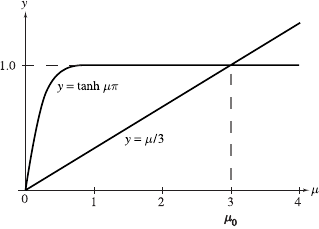
\includegraphics[scale=.8]{tanh.png}

En resumen, el problema con valores en la frontera (20)-(21) tiene un valor propio negativo $\lambda_{0}=-\mu_{0}^{2}$, tal que $\tan \mu_{0} \pi=\mu_{0} / 3$, y las funciones propias correspondientes son $y_{0}(x)=c_{0} \operatorname{senh} \mu_{0} x$, con $c_{0} \neq 0$ arbitrario.



{Ejemplo 3 (continuación)}
 

\textbf{Conclusión.} En el caso $\lambda<0$ el problema con valores en la frontera tiene un valor propio negativo 
$$\lambda_{0}=-\mu_{0}^{2},$$
tal que 
$$\tan \mu_{0} \pi=\mu_{0} / 3,$$
y las funciones propias correspondientes son 

$$y_{0}(x)=c_{0} \operatorname{senh} \mu_{0} x,\quad c_{0} \in\rr.$$ 

 


 

{Ejemplo 3 (continuación)}
\textbf{Caso 2. $\lambda=0$.} Cero es una raíz doble de la ecuación auxiliar, la solución general es:

$$y(x)=c_{1} x+c_{2}.$$ 

Al sustituir en las condiciones de contorno
$$
c_{2}=0, \quad 3 \pi c_{1}+3 c_{2}-c_{1}=0
$$
que tiene la solución $c_{1}=c_{2}=0$. 

No tenemos funciones propias.
 


 

{Ejemplo 3 (continuación)}
\textbf{Caso 3. $\lambda=\mu^{2}>0$  para $\mu>0$.} Raíces:

$$r=\pm \mu i,$$
Solución general: 

$$y(x)=c_{1} \cos \mu x+c_{2}\sen \mu x .$$

Sustituyenco en condiciones de contorno
$$
c_{1}=0, \quad 3\left(c_{1} \cos \mu \pi+c_{2} \operatorname{sen} \mu \pi\right)-\left(-\mu c_{1} \operatorname{sen} \mu \pi+\mu c_{2} \cos \mu \pi\right)=0 .
$$
$\mathrm{Al}$ hacer $c_{1}=0$ en la última ecuación, obtenemos
$$
c_{2}(3 \operatorname{sen} \mu \pi-\mu \cos \mu \pi)=0 .
$$
Para que existan soluciones no triviales, $\mu$ debe satisfacer 

$$\tan \mu \pi=\frac{1}{3} \mu.$$

 


 

{Ejemplo 3 (continuación)}
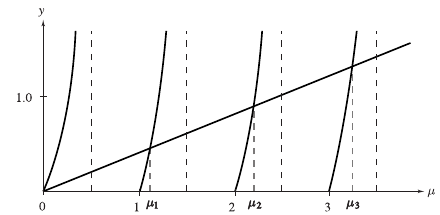
\includegraphics[scale=.6]{tanh2.png}

Hay una infinidad de soluciones $\mu_{1}<\mu_{2}<\ldots $ por ende de autovalores $\lambda_{n}=\mu_{n}^{2}, n=1,2,3, \ldots$ con autofunciones correspondientes  

$$y_{n}(x)=c_{2}\sen \mu_{n} x, \hbox{ con }c_{2} \neq 0,$$  






\section{Problemas regulares de Sturm-Liouville}



 

{Problemas regulares de Sturm-Liouville}

Retornemos al problema general de hallar los valores propios y funciones propias de:
\begin{empheq}[box=\tcbhighmath]{equation}\label{eq:sl_main2}  
\left\{
        \begin{array}{ll}
                    \frac{d}{d x}\left(p(x) \frac{d y}{d x}\right)+q(x) y+\lambda r(x) y=0, & a<x<b\\
                    a_{1} y(a)+a_{2} y^{\prime}(a)=0,&\\
                     b_{1} y(b)+b_{2} y^{\prime}(b)=0, &
        \end{array}
 \right.
\end{empheq}
donde
\begin{itemize}
 \item $p(x), p^{\prime}(x), q(x)$ y $r(x)$ son funciones continuas en $[a, b]$
 \item $p(x)>0$ y $r(x)>0$ en $[a, b]$.
 \item Se excluye el caso en que $a_{1}=a_{2}=0$ o $b_{1}=b_{2}=0$.
\end{itemize}   



\subsection{Llevando a la forma de Sturm-Liouville}



 

{Llevando a la forma de Sturm-Liouville}

\textbf{Disgresión:} cualquier ecuación de la forma 
\begin{equation}\label{eq:20gral}
    A_{2}(x) y^{\prime \prime}(x)+A_{1}(x) y^{\prime}(x)+A_{0}(x) y(x)+\lambda \rho(x) y(x)=0
\end{equation}
se puede convertir  en una ecuación del tipo que \eqref{eq:sl_main2}.



Debemos determinar $p$ de modo que 

$$\left(p y^{\prime}\right)^{\prime}=p y^{\prime \prime}+p^{\prime} y^{\prime}=A_{2} y^{\prime \prime}+A_{1}y^{\prime}.$$

Es decir 

$$p=A_{2},\quad p^{\prime}=A_{1}.$$
Pero en general, $A_{2}^{\prime} \neq A_{1}$, de modo que este método directo no siempre es aplicable.


 



 

{Llevando a la forma de Sturm-Liouville}

\tikz[baseline]{
      \node[fill=frametit, square,anchor=base] (t0)
           {Idea!}} Buscar
 \emph{factor integrante} $\mu(x)$ tal que al multiplicar \eqref{eq:20gral} por $\mu$,  obtenemos coeficientes tales que  $\left(\mu A_{2}\right)^{\prime}=\mu A_{1}$. 
 
 
 Lamemos $p=\mu A_{2}$,  queremos 
 
 $$p^{\prime}=\mu A_{1}=p A_{1} / A_{2}.$$
 
 Es una ecuación en variables separables. Resolviendo
$$
p(x)=C e^{\int A_{1}(x) / A_{2}( x) d x},\quad C\in\rr
$$

Tomamos $C=1$ 
$$\mu(x)=p / A_{2}=\left[1 / A_{2}(x)\right] e^{\int A_{1}(x) / A_{2}(x) d x}.$$

Al multiplicar \eqref{eq:20gral} por  $\mu$ se tiene

$$\left(p y^{\prime}\right)^{\prime}+q y+\lambda r y=0,$$

donde $p=\mu A_{2}, q=\mu A_{0} \mathrm{y} r=\mu \rho$. Necesitamos  que $A_{2}(x)\neq 0$



 



 

{Ejemplo}
 
 Convertir la siguiente ecuación a la forma de una ecuación de Sturm-Liouville:
$$
 3 x^{2} y''(x)+4 x y^{\prime}(x)+6 y(x)+\lambda y(x)=0, \quad x>0.
$$


\textbf{Solución.}  $A_{2}(x)=3 x^{2}$ y $A_{1}(x)=4 x$.
$$
\begin{aligned}
\mu(x) &=\frac{1}{3 x^{2}} e^{\int A_1(x) / A_2(x) d x}=\frac{1}{3 x^{2}} e^{\int(4 x)/3 x^{2} d x} \\
&=\frac{1}{3 x^{2}} e^{(4 / 3) \int x^{-1} d x}=\frac{1}{3 x^{2}} e^{(4 / 3) \ln x}=\frac{x^{4 / 3}}{3 x^{2}}=\frac{1}{3 x^{2 / 3}} .
\end{aligned}
$$
Al multiplicar la ecuación por $\mu(x)=1 /\left(3 x^{2 / 3}\right)$, obtenemos

$$\left(x^{4 / 3} y^{\prime}(x)\right)^{\prime}+2 x^{-2 / 3} y(x)+\lambda\left(3 x^{2 / 3}\right)^{-1} y(x)=0.$$



 


\subsection{Identidades Lagrange-Green}
 

{Identidad de Lagrange}
Definimos

$$\tikz[baseline]{
      \node[fill=frametit, square,anchor=base] (t0)
           {$ L\left[y](x):=\left(p(x) y^{\prime}(x)\right)^{\prime}+q(x) y(x)\right.$ }} $$
      
 la ecuación se escribe 
$$\tikz[baseline]{
      \node[fill=frametit, square,anchor=base] (t0)
           {$L[y](x)+\lambda r(x) y(x)=0 .$ }} 
$$


\begin{block}{Teorema [Identidad de lagrange]}  Sean $u$ y $v$ funciones con segundas derivadas continuas en el intervalo $[a, b]$. Entonces,

$$\tikz[baseline]{
      \node[fill=frametit, square,anchor=base] (t0)
           {$u L[v]-v L[u]=\frac{d}{d x}(p W[u, v]),$
    }} $$
donde el \emph{wronskiano} de $u$ y $v$ se define
$W[u, v]=u v^{\prime}-v u^{\prime}$  
\end{block}


 



{Identidad de Lagrange (Demostración)}

Usamos la regla del producto y sumamos y restamos $p u^{\prime} \boldsymbol{v}^{\prime}$ para tener
$$
\begin{aligned}
u L[v]-v L[u] &=u\left[\left(p v^{\prime}\right)^{\prime}+q v\right]-v\left[\left(p u^{\prime}\right)^{\prime}+q u\right] \\
&=u\left(p v^{\prime}\right)^{\prime}+q u v-v\left(p u^{\prime}\right)^{\prime}-q u v \\
&=u\left(p v^{\prime}\right)^{\prime}+u^{\prime}\left(p v^{\prime}\right)-v^{\prime}\left(p u^{\prime}\right)-v\left(p u^{\prime}\right)^{\prime} \\
&=\left[u\left(p v^{\prime}\right)\right]^{\prime}-\left[v\left(p u^{\prime}\right)\right]^{\prime} \\
&=\left[ p\left(u v^{\prime}-v u^{\prime}\right)\right]^{\prime} \\
&=\frac{d}{d x}[p W[u, v]]
\end{aligned}
$$



 



{Fórmula de Green}


\begin{block}{Corolario [Fórmula de Green]}
 Sean $u$ y $v$ funciones con segundas derivadas continuas en el intervalo $[a, b]$. Entonces,
 
 \begin{empheq}[box=\tcbhighmath]{equation}\label{eq:for_green_1}\int_{a}^{b}(u L[v]-v L[u])(x) d x=\left.(p W[u, v])(x)\right|_{a} ^{b}.
\end{empheq}
 
Si además u y $v$ satisfacen las condiciones en la frontera de \eqref{eq:sl_main2}, la fórmula de Green se simplifica a


\begin{empheq}[box=\tcbhighmath]{equation}\label{eq:for_green_2}\int_{a}^{b}(u L[v]-v L[u])(x) d x=0.
\end{empheq}
\end{block}


 



{Fórmula de Green (Demostración)}

La primera fórmula surge de integrar la identidad de Lagrange.

Para la segunda notar que si $a_{2} \neq 0$ y $b_{2} \neq 0$, entonces
$$
\begin{array}{ll}
u^{\prime}(a)=-\left(a_{1} / a_{2}\right) u(a), & u^{\prime}(b)=-\left(b_{1} / b_{2}\right) u(b) \\
v^{\prime}(a)=-\left(a_{1} / a_{2}\right) v(a), & v^{\prime}(b)=-\left(b_{1} / b_{2}\right) v(b)
\end{array}
$$
Al sustituir estos valores en el lado derecho de la primera fórmula
$$
\begin{aligned}
p(b) W & {[u, v](b)-p(a) W[u, v](a) } \\
=& p(b)\left[u(b) v^{\prime}(b)-u^{\prime}(b) v(b)\right]-p(a)\left[u(a) v^{\prime}(a)-u^{\prime}(a) v(a)\right] \\
=& p(b)\left[u(b)\left(-b_{1} / b_{2}\right) v(b)-\left(-b_{1} / b_{2}\right) u(b) v(b)\right] \\
& \quad-p(a)\left[u(a)\left(-a_{1} / a_{2}\right) v(a)-\left(-a_{1} / a_{2}\right) u(a) v(a)\right] \\
=& 0
\end{aligned}
$$




 



{Fórmula de Green (Demostración)}
 Cuando $a_{2}=0$ (de modo que $a_{1} \neq 0$ ), las condiciones de contorno implican que $u(a)$ y $v(a)$ se anulan. Por lo tanto, 
 $$\left[u(a) v^{\prime}(a)-u^{\prime}(a) v(a)\right]=0.$$
 De manera análoga, cuando $b_{2}=0$, obtenemos 
 $$\left[u(b) v^{\prime}(b)-u^{\prime}(b) v(b)\right]=0.$$\qed


\section{Operadores autoadjuntos}
\subsection{Definiciones}
{Producto interno}

\begin{block}{Producto interno}
Para $f,g\in L^2([a,b])$ se define

\begin{empheq}[box=\tcbhighmath]{equation}\label{eq:pro_int}
 (f, g)=\int_{a}^{b} f(x) g(x) d x.
\end{empheq}

entonces 

$$(\cdot, \cdot):L^2([a,b])\times L^2([a,b])\to\rr$$ 
es un producto interior en $L^2([a,b])$ 
\end{block}






{Autoadjunción} 
Ecuación \eqref{eq:for_green_2} Equivale

\begin{equation}\label{eq:autoadjunto}
 \tikz[baseline]{
      \node[fill=frametit] (t0)
           {$(u, L[v])=\left(L[u], v\right).$
    }}
\end{equation}


\begin{block}{Definición [Operadores autoadjuntos]} Un operador diferencial lineal $L$ que satisface \eqref{eq:autoadjunto} para todas las funciones $u$ y $v$ en su dominio se llama un \emph{operador autoadjunto. }
\end{block}



\textbf{Observación.} Hemos mostrado que si $L[y]=(py')'+qy$  y el dominio de $L$ es el conjunto de funciones que tienen segundas derivadas continuas en $[a, b]$ y satisfacen las condiciones en la frontera en \eqref{eq:sl_main2} , entonces $L$ es un operador autoadjunto.




\subsection{Autoadjunción $\Rightarrow \lambda\in\rr$}  
{Autoadjunción $\Rightarrow \lambda\in\rr$}

\begin{block}{Teorema} Los valores propios de un problema regular de Sturm-Liouville \eqref{eq:sl_main2}  son reales y tienen funciones propias con valores reales.
 
\end{block}


\textbf{Demostración.} Supongamos que $\lambda\in \mathbb{C}$ es un valor propio, con función propia $\phi(x)$, la que puede asumir valores complejos. Es decir,
$$L[\phi](x)+\lambda r(x) \phi(x)=0.$$

y $\phi\not\equiv 0$ satisface las condiciones en la frontera en  \eqref{eq:sl_main2}. Como $p, q$ y $r$ asumen valores reales, obtenemos
$$\overline{L[\phi](x)+\lambda r(x) \phi(x)}=L[\bar{\phi}](x)+\bar{\lambda} r(x) \bar{\phi}(x)=0$$
Como $a_{1}, a_{2}, b_{1}$ y $b_{2}$ son reales $\bar{\phi}$ también satisface las condiciones en la frontera en \eqref{eq:sl_main2}. Por lo tanto, $\bar{\lambda}$ es un valor propio con función propia $\bar{\phi}$




{Autoadjunción $\Rightarrow \lambda\in\rr$}

Por otro lado
$$\int_{a}^{b} L[\phi](x) \bar{\phi}(x) d x=-\lambda \int_{a}^{b} r(x) \phi(x) \bar{\phi}(x) d x=-\lambda \int_{a}^{b} r(x)|\phi(x)|^{2} d x.$$


Además por la segunda identidad de Green y el hecho de que $\bar{\lambda}$ sea un valor propio con función propia $\bar{\phi}$, vemos que


$$
\int_{a}^{b} L[\phi](x) \bar{\phi}(x) d x=\int_{a}^{b} \phi(x) L[\bar{\phi}](x) d x=-\bar{\lambda} \int_{a}^{b} r(x)|\phi(x)|^{2} d x
$$
Pero los lados izquierdos de las ecuaciones anteriores son los mismos, de modo que 
$$
-\lambda \int_{a}^{b} r(x)|\phi(x)|^{2} d x=-\bar{\lambda} \int_{a}^{b} r(x)|\phi(x)|^{2} d x
$$




{Autoadjunción $\Rightarrow \lambda\in\rr$}
Como $r(x)>0$ y $\phi\neq 0$, entonces 
$$\int_{a}^{b} r(x)|\phi(x)|^{2} d x>0.$$ 

Obtenemos $\lambda=\bar{\lambda}$, vale decir $\lambda\in\rr$. 

Tomando partes real e imaginaria de  $\phi$ obtenemos  funciones propias con valores reales correspondientes a $\lambda$.\qed 


\subsection{Multiplicidad de autovalores}

{Multiplicidad de autovalores}


\begin{block}{Definición [Autovalores simples]} Si todas las funciones propias asociadas a un valor propio particular son sólo múltiplos escalares entre sí, entonces el valor propio se llama \emph{simple}.
\end{block}


\begin{block}{Teorema [Autovalores simples]}
Todos los valores propios del problema regular de Sturm-Liouville con valores en la frontera \eqref{eq:sl_main2} son simples.
\end{block}



{Multiplicidad de autovalores}

\textbf{Demostración.} Si $\phi(x)$ y $\psi(x)$ son autofunciones  correspondientes a $\lambda$: 
$$
a_{1} \phi(a)+a_{2} \phi^{\prime}(a)=0, \quad a_{1} \psi(a)+a_{2} \psi^{\prime}(a)=0
$$
Supongamos que $a_{2} \neq 0$. ( si $a_{2}=0$ y $a_{1} \neq 0$ queda de \textbf{ejercicio}.) Despejando
$$
\phi^{\prime}(a)=\left(-a_{1} / a_{2}\right) \phi(a), \quad \psi^{\prime}(a)=\left(-a_{1} / a_{2}\right) \psi(a)
$$
Calculemos el wronskiano de $\phi$ y $\psi$ en $x=a$
$$
\begin{aligned}
W[\phi, \psi](a) &=\phi(a) \psi^{\prime}(a)-\phi^{\prime}(a) \psi(a) \\
&=\phi(a)\left(-a_{1} / a_{2}\right) \psi(a)-\left(-a_{1} / a_{2}\right) \phi(a) \psi(a)=0
\end{aligned}
$$
Si el wronskiano de dos soluciones de una ecuación lineal homogénea de segundo orden se anula en un punto, entonces las dos soluciones son linealmente dependientes. Así, $\lambda$ es un valor propio simple.\qed



\subsection{Ortogonalidad}

{Ortogonalidad}
\begin{block}{Teorema [Ortogonalidad]} Las funciones propias que corresponden a valores propios distintos
de un problema regular de Sturm-Liouville con valores en la frontera \eqref{eq:sl_main2} son \emph{ortogonales} con respecto de la función de ponderación $r(x)$ en $[a, b]$. Vale decir si $\phi$ y $\psi$ son autofunciones asociadas a los autovalores $\lambda$ y $\mu$ con $\lambda\neq \mu$ entonces

\begin{empheq}[box=\tcbhighmath]{equation}\label{eq:ortogo}
 \int_{a}^{b} \phi(x) \psi(x) r(x) d x=0.
\end{empheq} 
\end{block}

 


{Ortogonalidad}


\textbf{Demostración.} Tenemos

$$L[\phi]=-\lambda r \phi\quad\hbox{ y }\quad L[\psi]=-\mu r \psi.$$

Podemos suponer que $\phi$ y $\psi$ tienen valores reales. Por la fórmula de Green
$$
\begin{aligned}
0 &=\int_{a}^{b}(\phi L[\psi]-\psi L[\phi])(x) d x \\
&=\int_{a}^{b}(-\phi \mu r \psi+\psi \lambda r \phi)(x) d x \\
&=(\lambda-\mu) \int_{a}^{b} \phi(x) \psi(x) r(x) d x
\end{aligned}
$$
Como $\lambda \neq \mu$, tenemos
$$
\int_{a}^{b} \phi(x) \psi(x) r(x) d x=0
$$
\qed
 


{Ortogonalidad, Ejemplo}

\textbf{Ejercicio} Demostrar que el problema
$$y^{\prime \prime}+\lambda y=0 ; \quad y(0)=y(\pi)=0$$

tiene autovalores  $\lambda_{n}=n^{2}, n=1,2$, $3, \ldots$, con funciones propias correspondientes $\phi_{n}(x)=c_{n}$ sen $n x$. Verificar la ortogonalidad de manera directa.

 
 
 
 \subsection{Desarrollo en serie de autofunciones}
 
 {Infinitud de autovalores}
 

 \begin{block}{Teorema} Los valores propios del problema regular de Sturm-Liouville con valores en la frontera \eqref{eq:sl_main2} forman una sucesión numerable y creciente
$$\lambda_{1}<\lambda_{2}<\lambda_{3}<\cdots$$
con:
$$\lim _{n \rightarrow \infty} \lambda_{n}=+\infty.$$
\end{block}



\textbf{Demostración}. Será omitida, ver por ejemplo Garrett Birkhoff y Gian-Carlo Rota. Ordinary Differential Equations



 {Desarrollos en serie}
 Si $\lambda_{1}<\lambda_{2}<\lambda_{3}<\cdots$ son valores propios del problema \eqref{eq:sl_main2} con funciones propias  $\left\{\phi_{n}(x)\right\}_{n=1}^{\infty}$,  ortonormales respecto  a $r(x)$ en $[a, b]$:

 $$\int_{a}^{b} \phi_{n}(x) \phi_{m}(x) r(x) d x= \begin{cases}0, & m \neq n, \\ 1, & m=n,\end{cases}.$$ 

En la unidad 7 vimos como asociar a una función  $f$ un desarrollo ortogonal 

\begin{empheq}[box=\tcbhighmath]{equation}\label{eq:des_ortogo}
f(x) \sim \sum_{n=1}^{\infty} c_{n} \phi_{n}(x),
\end{empheq}

donde

\begin{empheq}[box=\tcbhighmath]{equation}\label{eq:coef_fou}
c_{n}=\int_{a}^{b} f(x) \phi_{n}(x) r(x) d x.
\end{empheq}



 {Ortonormalización}


 \textbf{Observación} Podemos usar las funciones propias para formar un \emph{sistema ortonormal} con respecto de $r(x)$,  normalizando a cada función propia $\phi_{n}$, de modo que
$$\int_{a}^{b} \phi_{n}^{2}(x) r(x) d x=1.$$



\textbf{Ejercicio}  Considerar el problema de Sturm-Liouville con valores en la 
$$y^{\prime \prime}+\lambda y=0 ; \quad y(0)=0, \quad y^{\prime}(\pi)=0.$$

\begin{itemize}
 \item $\lambda_{n}=$ $(2 n-1)^{2} / 4, n=1,2,3, \ldots$ valores propios.
 \item $
\phi_{n}(x)=a_{n} \operatorname{sen}\left(\frac{2 n-1}{2}\right) x
$ funciones propias ortogonles respecto $r(x) \equiv 1$ en $[0, \pi]$.
\item Si $a_{n}=\sqrt{2 / \pi}$ el sistema es ortonormal.
\end{itemize}



 {Desarrollos en serie}
 
 \begin{block}{Teorema}  Sea $\left\{\phi_{n}\right\}_{n=1}^{\infty}$ un sistema ortonormal de funciones propias para el problema regular de Sturm-Liouville con valores en la frontera \eqref{eq:sl_main2}, entonces $\left\{\phi_{n}\right\}_{n=1}^{\infty}$ es completo en el conjunto de funciones continuas de cuadrado integrable en $[a,b]$, es decir si $f$ es continua:
  $$f(x)=\sum_{n=1}^{\infty} c_{n} \phi_{n}(x), \quad a \leq x \leq b,$$
  donde la convergencia de la serie es en media. Si además $f^{\prime}$ continua por partes  en $[a, b]$ y satisface las condiciones en la frontera la serie converge uniformemente en $[a, b]$.
 \end{block}
 
 
 \textbf{Demostración.}  Será omitida, ver por ejemplo Garrett Birkhoff y Gian-Carlo Rota. Ordinary Differential Equations
 

 {Desarrollos en serie}
Expresar
$$\small
f(x)= \begin{cases}2 x / \pi, & 0 \leq x \leq \pi / 2 \\ 1, & \pi / 2 \leq x \leq \pi\end{cases}
$$
mediante  el sistema:
$$\small
\phi_{n}(x)=\sqrt{\frac{2}{\pi}}\operatorname{sen}\left(\frac{2 n-1}{2}\right) x. $$ 
$$\small
\begin{aligned}
c_{n}=& \int_{0}^{\pi} f(x) \sqrt{2 / \pi} \operatorname{sen}\left(\frac{2 n-1}{2} x\right) d x \\
=&\left(\frac{2}{\pi}\right)^{3 / 2} \int_{0}^{\pi / 2} x \operatorname{sen}\left(\frac{2 n-1}{2} x\right) d x+\left(\frac{2}{\pi}\right)^{1 / 2} \int_{\pi / 2}^{\pi} \operatorname{sen}\left(\frac{2 n-1}{2} x\right) d x \\
=&\left.\left(\frac{2}{\pi}\right)^{3 / 2}\left[\frac{-2 x}{2 n-1} \cos \left(\frac{2 n-1}{2} x\right)+\frac{4}{(2 n-1)^{2}} \operatorname{sen}\left(\frac{2 n-1}{2} x\right)\right]\right|_{0} ^{\pi / 2} \\
&-\left.\left(\frac{2}{\pi}\right)^{1 / 2}\left[\frac{2}{2 n-1} \cos \left(\frac{2 n-1}{2} x\right)\right]\right|_{\pi / 2} ^{\pi},
\end{aligned}
$$
 

 {Desarrollos en serie}
 
 Entonces 
$$c_{n}=\frac{2^{7 / 2}}{\pi^{3 / 2}(2 n-1)^{2}} \operatorname{sen}\left(\frac{n \pi}{2}-\frac{\pi}{4}\right),\quad n=1,2,3, \ldots .$$
Por lo tanto,
$$\small
\begin{aligned}
f(x) &=\sum_{n=1}^{\infty} c_{n} \sqrt{2} / \pi \operatorname{sen}\left(\frac{2 n-1}{2} x\right) \\
&=\frac{2^{7 / 2}}{\pi^{2}} \operatorname{sen}(x / 2)+\frac{2^{7 / 2}}{9 \pi^{2}} \operatorname{sen}(3 x / 2)-\frac{2^{7 / 2}}{25 \pi^{2}} \operatorname{sen}(5 x / 2)-\frac{2^{7 / 2}}{49 \pi^{2}} \operatorname{sen}(7 x / 2)+\cdots,
\end{aligned}
$$
 Como $f(0)=0$ y $f^{\prime}(\pi)=0, f$ satisface las condiciones en la frontera. Además, $f$ es continua y $f^{\prime}$ es continua por partes en $[0, \pi]$. Por lo tanto, la serie en converge uniformemente a $f$ en $[0, \pi]$.


 

 {Otro resultado de convergencia}

\begin{block}{Teorema} Sea $\left\{\phi_{n}\right\}_{n=1}^{\infty}$ una sucesión ortonormal de funciones propias para el problema regular de Sturm-Liouville con valores en la frontera \eqref{eq:sl_main2}. Sean $f$ y $f^{\prime}$ continuas por partes en $[a, b]$. Entonces, para cualquier $x$ en $(a, b)$,
\begin{empheq}[box=\tcbhighmath]{equation}\label{eq:conv_dis}
\sum_{n=1}^{\infty} c_{n} \phi_{n}(x)=\frac{1}{2}\left[f\left(x^{+}\right)+f\left(x^{-}\right)\right],
\end{empheq}
donde las $c_{n}$ están dadas por la fórmula \eqref{eq:coef_fou}. 
\end{block}
 


\section{Aplicaciones}

\subsection{Vibraciones longitudinales de barras}
 
{Ecuación vibraciones longitudinales}


\emph{Bibliografía}
Charles Henry Edwards y David E. Penney. \emph{Ecuaciones diferenciales y problemas con valores en la frontera}.


\begin{itemize}
    \item Cuerda elástica situada en el intervalo $[0,L]$ del eje $x$ cuando no está estirada con área de sección transversal $A$ y densidad $\delta$.
    \itemSolo hay vibraciones longitudinales de la cuerda. $u(x, t):$  desplazamiento de la sección transversal  en el tiempo $t$, cuya posición es $x$ cuando la barra no está estirada. La posición en el tiempo $t$ de la sección transversal $x$ es $x+u(x, t)$.
\end{itemize}


\begin{center}
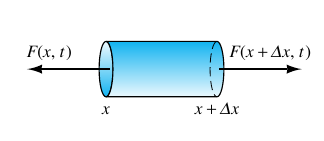
\includegraphics[scale=.5]{barra.png}
\end{center}



Por la \emph{Ley de Hooke} existe una constante $E$, tal que la fuerza $F(x, t)$ ejercida por la barra   es
$$
F(x, t)=-A E u_{x}(x, t).
$$
 

 
{Ecuación vibraciones longitudinales}

Por la \emph{Ley Balance Momentos}

$$
\begin{aligned}
(\delta A \Delta x) u_{t t}(\bar{x}, t)  \approx-F(x+\Delta x, t)+F(x, t) 
=A E\left[u_{x}(x+\Delta x, t)-u_{x}(x, t)\right]
\end{aligned}
$$
donde $\bar{x}$ representa el punto medio de $[x, x,+\Delta x]$. Cuando se divide la expresión entre $\delta A \Delta x$ y se toma el límite conforme $\Delta x \rightarrow 0$, el resultado es la ecuación de onda de una dimensión
$$
\frac{\partial^{2} u}{\partial t^{2}}=a^{2} \frac{\partial^{2} u}{\partial x^{2}}
$$
donde
$$
a^{2}=\frac{E}{\delta}
$$

 

 
{Ejemplo vibraciones longitudinales}

Supongamos una cuerda  donde su extremo $x=0$ está fijo y una masa $m$ está adherida a su otro extremo que es libre. 

\begin{center}
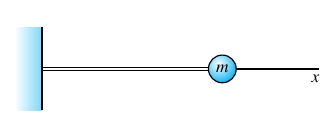
\includegraphics[scale=.4]{barra2.png}
\end{center}



Inicialmente la barra está estirada linealmente de tal manera que la sección transversal $x$ de la barra está  desplazada a $b x$. En el tiempo $t=0$ el sistema se pone en libertad partiendo del reposo. Debe resolverse el problema con valores en la frontera
$$
\left\{
\begin{aligned}
u_{t} &=a^{2} u_{x x} \quad(0<x<L, t>0) \\
u(0, t) &=0 \\
m u_{t t}(L, t) &=-A E u_{x}(L, t) \\
u(x, 0) &=b x, \quad u_{t}(x, 0)=0
\end{aligned}
\right.
$$
 

 
{Ejemplo vibraciones longitudinales}

 La sustitución de $u(x, t)=X(x) T(t)$ en $u_{t t}=a^{2} u_{x x}$ lleva, como es usual, a las ecuaciones
$$
X^{\prime \prime}+\lambda X=0, \quad T^{\prime \prime}+\lambda a^{2} T=0
$$


La condición de frontera implica 
$$u(0, t)=X(0) T(t)=0,$$

y esto que

$$X(0)=0.$$


Debido a que $u_{t t}=X T^{\prime \prime}$ y $u_{x}=$ $X^{\prime} T$, reemplazando en la condición de cotorno para $x=L$  
$$
m X(L) T^{\prime \prime}(t)=-A E X^{\prime}(L) T(t)
$$
como la otra condición de la frontera. 

 

 
{Ejemplo vibraciones longitudinales}


La sustitución de
$$
T^{\prime \prime}(t)=-\lambda a^{2} T(t)=-\frac{\lambda E}{\delta} T(t)
$$
seguida por la división entre $-E T(t) / \delta$, resulta en 
$$m \lambda X(L)=A \delta X^{\prime}(L).$$


Así, el problema de autovalores para $X(x)$ es
$$
\left\{
\begin{array}{l}
X^{\prime \prime}+\lambda X=0 \\
X(0)=0, \quad m \lambda X(L)=A \delta X^{\prime}(L)
\end{array}
\right.
$$

Debido a la presencia de $\lambda$ en la condición de frontera derecha  éste \emph{no es un problema de Sturm-Liouville}, por lo que los teoremas que hemos establecido lamentablemente no aplican. 

No obstante, todos los eigenvalores  son positivos (\textbf{ejercicio}), por tanto, se escribe $\lambda=\alpha^{2}$.



 

 
{Ejemplo vibraciones longitudinales}

De la condición de frontera izquierda inferimos
$$X(x)=\operatorname{sen} \alpha x.$$ 


De la condición de frontera derecha 
$$
m \alpha^{2} \operatorname{sen} \alpha L=A \delta \alpha \cos \alpha L
$$
y así
$$
\tan \alpha L=\frac{A \delta}{m \alpha}=\frac{M / m}{\alpha L}
$$



donde  $M=A \delta L$ es la masa total y $\beta:=\alpha L$.
Luego  los autovalores y sus autofunciones asociadas son
$$
\lambda_{n}=\frac{\beta_{n}^{2}}{L^{2}}, \quad X_{n}(x)=\operatorname{sen} \frac{\beta_{n} x}{L}
$$
para $n=1,2,3, \ldots$, donde $\left\{\beta_{n}\right\}^{\infty}_1$ son las raíces positivas de la ecuación
$$
\tan x=\frac{M / m}{x},
$$

 

 
{Ejemplo vibraciones longitudinales}
\begin{center}
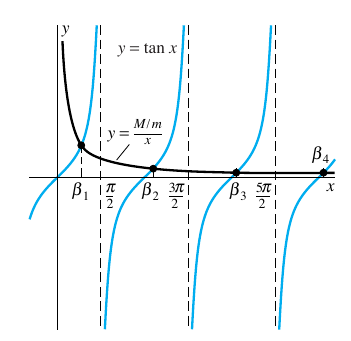
\includegraphics[scale=.8]{barra3.png}
\end{center}

 

 
{Ejemplo vibraciones longitudinales}

Continuando 
$$\small
T_{n}^{\prime \prime}+\frac{\beta_{n}^{2} a^{2}}{L^{2}} T_{n}=0, \quad T_{n}^{\prime}(0)=0
$$
Asi
$$\small T_{n}(t)=\cos \left(\beta_{n} a t / L\right).$$



Sólo falta encontrar los coeficientes $\left\{c_{n}\right\}_{1}^{\infty}$ de tal manera que la serie
$$\small
u(x, t)=\sum_{n=1}^{\infty} c_{n} \cos \frac{\beta_{n} a t}{L} \operatorname{sen} \frac{\beta_{n} x}{L}
$$
satisfaga la condición no homogénea
$$\small
u(x, 0)=\sum_{n=1}^{\infty} c_{n} \operatorname{sen} \frac{\beta_{n} x}{L}=f(x)=b x .
$$


En este ejemplo las autofunciones $\left\{\operatorname{sen}\left(\beta_{n} x / L\right)\right\}_{1}^{\infty}$ no son ortogonales en el intervalo $[0, L]$ con respecto al peso $r(x) \equiv 1$ (\textbf{ejercicio}), de  modo que la  fórmula para los coeficientes no aplica.
 

 
 
 \section{Problemas singulares de Sturm-Liouville}
 
 \subsection{Definición y ejemplos}
{Problemas singulares de Sturm-Liouville}
Supongamos el operador
$$L[y](x):=\frac{d}{d x}\left[p(x) \frac{d y}{d x}\right]+q(x) y$$
y consideremos la ecuación
 $$\quad L[y](x)+\lambda r(x) y(x)=0, \quad a<x<b.$$
donde  $p(x), p^{\prime}(x), q(x)$ y $r(x)$ son  continuas en $(a, b)$ con valores reales, y además $p(x)$ y $r(x)$ son positivas en $(a, b)$. Llamamos a la ecuación  una ecuación \emph{singular de Sturm-Liouville}  si una  de las siguientes situaciones ocurren:

\begin{itemize}
 \item $\lim _{x \to a^{+}} p(x)=0 \circ \lim _{x\to b^-}(x)=0$.
 \item $p(x), q(x)$ o $r(x)$ se vuelven no acotadas cuando $x$ tiende a $a$ o $b$.
 \item El intervalo $(a, b)$ no está acotado (por ejemplo, $(a, \infty),(-\infty, b)$ o $(-\infty, \infty))$.
\end{itemize}






 
  
{Ejemplos: Ecuación Bessel}

La \emph{ecuación de Bessel de orden $\nu$}
\begin{empheq}[box=\tcbhighmath]{equation}\label{eq:bessel}  
 t^{2} y^{\prime \prime}(t)+y^{\prime}(t)+\left(t^{2}-\nu^{2}\right) y=0, \quad 0<t<\sqrt{\lambda} b
\end{empheq}
 
se puede transformar mediante la sustitución $t=\sqrt{\lambda} x$ en la ecuación singular de Sturm-Liouville

\begin{empheq}[box=\tcbhighmath]{equation}\label{eq:bessel2}  
\frac{d}{d x}\left[x \frac{d y}{d x}\right]-\frac{\nu^{2}}{x} y+\lambda x y=0, \quad 0<x<b.
\end{empheq}


En este caso, $p(x)=x$, que se anula para $x=0$. Además, para $\nu \neq 0$, la función $q(x)=-\nu^{2} / x$ no está acotada cuando $x \rightarrow 0^{+}$.





 
  
{Ejemplos: Ecuación de Legendre}

\begin{empheq}[box=\tcbhighmath]{equation}\label{eq:legendre}  \left(1-x^{2}\right) y^{\prime \prime}-2 x y^{\prime}+n(n+1) y=0, \quad-1<x<1
\end{empheq}

se puede escribir como la ecuación singular de Sturm-Liouville


\begin{empheq}[box=\tcbhighmath]{equation}\label{eq:legendre2} 
\frac{d}{d x}\left[\left(1-x^{2}\right) \frac{d y}{d x}\right]+\lambda y=0, \quad-1<x<1,
\end{empheq}
donde $\lambda=n(n+1)$. En este caso, $p(x)=1-x^{2}$ se anula en los dos extremos $\pm 1$.





 
  
{Ejemplos: Ecuación de Hermite}

\begin{empheq}[box=\tcbhighmath]{equation}\label{eq:hermite1}  
 y^{\prime \prime}-2 x y^{\prime}+2 n y=0, \quad-\infty<x<\infty,
\end{empheq}
al ser multiplicada por $e^{-x^{2}}$, se convierte en la ecuación singular de Sturm-Liouville



\begin{empheq}[box=\tcbhighmath]{equation}\label{eq:hermite1}  
 \frac{d}{d x}\left[e^{-x^{2}} \frac{d y}{d x}\right]+\lambda e^{-x^{2}} y=0, \quad-\infty<x<\infty,
\end{empheq}
donde $\lambda=2 n$. En este caso, el intervalo $(-\infty, \infty)$ no está acotado.







 
\subsection{Autoadjunción}
{Autoadjunción}

¿Cuáles condiciones en la frontera convierten a una ecuación singular de Sturm-Liouville en un problema autoadjunto?

Debemos tener
$$
\int_{a}^{b}(u L[v]-v L[u])(x) d x=\lim _{x \rightarrow b} p(x) W[u, v](x)-\lim _{x \rightarrow a^{+}} p(x) W[ u, v](x) .
$$
 
\begin{empheq}[box=\tcbhighmath]{multline}\label{eq:cond_suf}  
\lim _{x \rightarrow a^{+}} p(x)\left[u(x) v^{\prime}(x)-u^{\prime}(x) v(x)\right]\\=\lim _{x \rightarrow b^{-}} p(x)\left[u(x) v^{\prime}(x)-u^{\prime}(x) v(x)\right]=0
\end{empheq}





 
  
{Condiciones singulares en la frontera}



\begin{block}{Lema} Cualquiera de las  condiciones siguientes garantizan la ecuación \eqref{eq:cond_suf} en $a$:
    \begin{enumerate}
        \item $\lim _{x \rightarrow a^{+}} p(x)=p(a)$ existe y $u, v$ satisfacen la condición en la frontera
            \begin{equation}\label{eq:con_cont_1}
            a_{1} y(a)+a_{2} y^{\prime}(a)=0,\hbox{ con  }a_{1}, a_{2} \hbox{ no ambos nulos.}
            \end{equation}

        \item$\lim_{x\to a^+}p(x)=0$ y $u, v$ satisfacen la condición en la frontera
            \begin{equation}\label{eq:con_cont_2}
                y(x), y^{\prime}(x) \hbox{ permanecen acotados cuando } x \rightarrow a^{+}.
            \end{equation} 
        \item Las funciones $u, v$ satisfacen la condición en la frontera
            \begin{equation}\label{eq:con_cont_3}
                \lim _{x \rightarrow a^{+}} \sqrt{p(x)} y(x)=0 \hbox{ y }\lim _{x \rightarrow a^{+}} \sqrt{p(x)} y^{\prime}(x)=0
            \end{equation}
       \end{enumerate}
\end{block}





 
  
{Condiciones singulares en la frontera}


\textbf{Demostración.}

(1) Sin pérdida de generalidad, suponemos que $a_{1} \neq 0$, Entonces,  implica que $u(a)=-\left(a_{2} / a_{1}\right) u^{\prime}(a)$ y $v(a)=-\left(a_{2} / a_{1}\right) v^{\prime}(a)$. Al sustituir

$$
\begin{aligned}
p(a)\left[u(a) v^{\prime}(a)-u^{\prime}(a) v(a)\right] &=p(a)\left[-\left(a_{2} / a_{1}\right) u^{\prime}(a) v^{\prime}(a)+\left(a_{2} / a_{1}\right) u^{\prime}(a) v^{\prime}(a)\right] \\
&=0
\end{aligned}
$$


(2)  Si $u, u^{\prime}, v$ y $ v^{\prime}$ permanecen acotadas cuando $x$ tiende a $a$ por la derecha, entonces  $W[u,v]$ permanece acotado. Como $\lim_{x \rightarrow a^{+}} p(x)=0$ y el producto de un factor acotado, por un factor que tiende a cero tiende a cero,  se cumple \eqref{eq:cond_suf}.





 
  
{Condiciones singulares en la frontera}

(3) Si $u$ y $v$ satisfacen \eqref{eq:con_cont_3}, entonces 
$$
\begin{aligned}
\lim _{x \rightarrow a^{+}} p(x)\left[u(x) v^{\prime}(x)-u^{\prime}(x) v(x)\right]=&\left(\lim _{x \rightarrow a^{+}} \sqrt{p(x)} u(x)\right)\left(\lim _{x \rightarrow a^{\prime}} \sqrt{p(x)} v^{\prime}(x)\right) \\
&-\left(\lim _{x \rightarrow a^{+}} \sqrt{p(x)} u^{\prime}(x)\right)\left(\lim _{x \rightarrow a^{+}} \sqrt{p(x)} v(x)\right) \\
=& 0-0=0 .
\end{aligned}
$$
Por lo tanto, se cumple la ecuación \eqref{eq:cond_suf}.


Se puede establecer  similarmente las mismas afirmaciones para el punto $b$ 

 

 \subsection{ Ecuación de Bessel}
 
{Ejemplo: Ecuación de Bessel}
 
Un problema singular de Sturm-Liouville con valores en la frontera típico asociado a la ecuación de Bessel de orden $\nu$ es

\begin{empheq}[box=\tcbhighmath,left=\left\{,right=\right.]{align}  
        \frac{d}{d x}\left[x \frac{d y}{d x}\right]-\frac{\nu^{2}}{x} y+\lambda x y=0, \quad 0<x<1.\\
        y(x), y^{\prime}(x) \hbox{ permanecen acotadas cuando } x \rightarrow 0^{+},\\
        y(1)=0.
\end{empheq}


Este problema es autoadjunto, pues la condición (2) del lema  se cumple en $a=0$ y  la condición (1)  se cumple en $b=1$.

Si $\lambda>0$, la sustitución $t=\sqrt{\lambda} x$ transforma la  ecuación en la ecuación de  Bessel 
\begin{empheq}[box=\tcbhighmath]{multline*}  
t^{2} y^{\prime \prime}+t y^{\prime}+\left(t^{2}-\nu^{2}\right) y=0.
\end{empheq}
 

{Ejemplo: Ecuación de Bessel}

En cursos básicos de ecuaciones diferenciales se demuestra que la solución general se escribe
\begin{empheq}[box=\tcbhighmath]{multline*}  
y(t)=c_{1} J_{\nu}(t)+c_{2} Y_{\nu}(t)
\end{empheq}
o
$$
y(x)=c_{1} J_{\nu}(\sqrt{\lambda} x)+c_{2} Y_{\nu}(\sqrt{\lambda} x)
$$



\begin{itemize}
 \item $J_{\nu}$ se llama \emph{Función de Bessel de primera especie} y satisface las hipótesis (2) del Lema en $x=0$ para $\nu=0$ y $\nu\geq 1$.
 \item $Y_{\nu}$ se llama \emph{Función de Bessel de segunda especie} y no está acotada cerca de $x=0$.
\end{itemize}

 

{Ejemplo: Ecuación de Bessel}


Para que se cumpla  la condición de contorno en $x=0$ debemos tener $c_{2}=0$ 

Para que se cumpla la condición de contorno en $x=1$  con $y(x)=c_{1} J_{\nu}(\sqrt{\lambda} x)$, necesitamos que $c_{1}=0$ o 
$$
J_{\nu}(\sqrt{\lambda} )=0
$$
 
 
 
\begin{block}{Teorema} 
La función de Bessel $J_{\nu}$ tiene una sucesión creciente de ceros reales:
$$
0<\alpha_{\nu 1}<\alpha_{\nu 2}<\alpha_{\nu 3}<\cdots
$$
\end{block}

 

{Ejemplo: Ecuación de Bessel}

Por lo tanto, 

$$\lambda_{\nu n}=\alpha_{\nu n}{ }^{2}, \nu,n=0,1,2,3, \ldots$$
 son valores propios  con funciones propias correspondientes
$$y_{\nu n}(x)=c_{1} J_{\nu}\left(\alpha_{\nu n} x\right).$$

Éstos son los únicos valores propios positivos. Además, se puede mostrar que no existen valores propios no positivos.



Las funciones propias en  son ortogonales con respecto de la función de ponderación $r(x)=x$ :

\begin{empheq}[box=\tcbhighmath]{multline*}  
\int_{0}^{1} J_{\nu}\left(\alpha_{\nu n} x\right) J_{\nu}\left(\alpha_{\nu m} x\right) x d x=0, \quad n \neq m
\end{empheq}




{Ejemplo: Ecuación de Bessel}


Si $f(x)$ es una función dada, entonces un desarrollo mediante funciones propias asociado a $f$ es
\begin{empheq}[box=\tcbhighmath]{multline*}  
f \sim \sum_{n=1}^{\infty} a_{n} J_{\nu}\left(\alpha_{v n} x\right)
\end{empheq}

donde
\begin{empheq}[box=\tcbhighmath]{multline*}  
a_{n}=\frac{\int_{0}^{1} f(x) J_{\nu}\left(\alpha_{\nu n} x\right) x d x}{\int_{0}^{1} J_{v}^{2}\left(\alpha_{\nu n} x\right) x d x}, \quad n=1,2,3, \ldots
\end{empheq}


Cuando $f$ y $f^{\prime}$ son continuas por partes en $[0,1]$, el desarrollo en converge a 
$$\left[f\left(x^{+}\right)+f\left(x^{-}\right)\right] / 2$$ 

para cada $x$ en $(0,1)$.



\subsection{Ecuación de Legendre} 
{Ejemplo: Ecuación de Legendre} 

Un problema singular de Sturm-Liouville con valores en la frontera típico asociado a la \emph{ecuación de Legendre} es

\begin{empheq}[box=\tcbhighmath,left=\left\{,right=\right.]{align}  
            \frac{d}{d x}\left[\left(1-x^{2}\right) \frac{d y}{d x}\right]+\lambda y=0, \quad-1<x<1\\
            y(x), y^{\prime}(x) \hbox{ permanecen acotadas cuando } x \rightarrow \pm 1.
\end{empheq}


Es autoadjunto, pues se cumple  la condición (2) del lema  en $x=\pm 1$. 

En cursos de ecuaciones diferenciales ordinarias se ve que la ecuación  tiene soluciones polinomiales para $\lambda=n(n+1), n=0,1,2, \ldots$.  Estas soluciones son múltiplos constantes de los \emph{polinomios de Legendre}
\begin{empheq}[box=\tcbhighmath]{multline*}  
P_{n}(x)=2^{-n} \sum_{m=0}^{[n / 2]} \frac{(-1)^{m}(2 n-2 m) !}{(n-m) ! m !(n-2 m) !} x^{n-2 m}
\end{empheq}
donde $[n / 2]$ es la parte entera.



{Ejemplo: Ecuación de Legendre} 

  $P_{n}(x)$ son ortogonales en $[-1,1]$ con respecto de $r(x)=1$ :
 
\begin{empheq}[box=\tcbhighmath]{multline*}  
\int_{-1}^{1} P_{n}(x) P_{m}(x) d x=0, \quad n \neq m
\end{empheq}



Si $f(x)$ es una función dada, entonces un desarrollo mediante funciones propias para $f(x)$, en términos de los polinomios de Legendre es

\begin{empheq}[box=\tcbhighmath]{multline*}  
 f \sim \sum_{n=0}^{\infty} a_{n} P_{n}(x),
\end{empheq}
 
donde
\begin{empheq}[box=\tcbhighmath]{multline*}  
a_{n}=\frac{\int_{-1}^{1} f(x) P_{n}(x) d x}{\int_{-1}^{1} P_{n}^{2}(x) d x}, \quad n=0,1,2, \ldots
\end{empheq}


Los resultados de convergencia similares a los dados para series de Fourier se cumplen para este desarrollo. 



\subsection{Ecuación de Hermite}
{Ejemplo: Ecuación de Hermite}

Un problema singular de Sturm-Liouville con valores en la frontera asociado a la ecuación de Hermite es
\begin{empheq}[box=\tcbhighmath,left=\left\{,right=\right.]{align}  
     \frac{d}{d x}\left[e^{-x^{2}} \frac{d y}{d x}\right]+\lambda e^{-x^{2}} y=0, \quad-\infty<x<\infty\\
    \lim _{x \rightarrow+\infty} e^{-x^{2} / 2} y(x)=0 \hbox{ y } \lim _{x \rightarrow+\infty} e^{-x^{2} / 2} y^{\prime}(x)=0.
\end{empheq}
Por la condición (3) del lema , el operador lineal asociado al problema es autoadjunto.


Se puede demostrar que se puede transformar la ecuación del problema en  la ecuación de Hermite 

$$y^{\prime \prime}-2 x y^{\prime}+2 n y=0.$$

También que esta ecuación tiene soluciones polinomiales que son múltiplos constantes de los \emph{polinomios de Hermite $H_{n}(x), n=0,1,2, \ldots$ 
}


{Ejemplo: Ecuación de Hermite}
Las soluciones polinomiales son las únicas que satisfacen las condiciones en la frontera. Se deduce que los valores propios son $\lambda_{n}=2 n, n=0,1,2, \ldots$, con funciones propias correspondientes $H_{n}(x)$. 


Los polinomios de Hermite $H_{n}(x)$ son ortogonales en $(-\infty, \infty)$ con respecto de la función de ponderación $r(x)=e^{-x^{2}}$ :

\begin{empheq}[box=\tcbhighmath]{equation}  
    \int_{-\infty}^{\infty} H_{n}(x) H_{m}(x) e^{-x^{2}} d x=0, \quad n \neq m.
\end{empheq}




{Ejemplo: Ecuación de Hermite}
Si $f$ es una función dada, entonces un desarrollo con funciones propias asociado a $f$ está dado por
$$f \sim \sum_{n=0}^{\infty} a_{n} H_{n}(x)$$ 
donde
$$
a_{n}=\frac{\int_{-\infty}^{\infty} f(x) H_{n}(x) e^{-x^{2}} d x}{\int_{-\infty}^{\infty} H_{n}^{2}(x) e^{-x^{2}} d x}, \quad n=0,1,2, \ldots
$$

 

 \subsection{Aplicaciones}
 


{Vibraciones transversales de una membrana elástica}
Membrana elástica, por ejemplo un tambor, que es mantenida fija a un arocircular. 
Viene gobernada por la ecuación de \emph{ondas bidimensional}

\[ u_{tt}=\Delta u:=u_{xx}+u_{yy}\]

\begin{figure}
    \begin{center}
        \animategraphics[autoplay , scale=.25,loop=true]{15}{/home/fernando/fer/Docencia/grado/EcuacionesDiferenciales/Materiales/Teoria_Basica/membrana/12/mem-}{0}{49}
    \end{center}  
\caption{Membrana vibrante}
\end{figure}
 

{Variables y suposiciones}


\textbf{Variables}

\begin{itemize}
 \item$t$ es el tiempo,
 \item $x,y,u$ son las coordenadas de un punto sobre la membrana en un sistema de coordenadas cartesiano ortogonal.

\end{itemize}



\textbf{Suposiciones.}
\begin{itemize}
 \item No actúa otra fuerza más que la tensión de la membrana.
 \itemEl material de esta membrana es uniforme.
 \itemLa dirección de desplazamientos de un punto sobre la membrana es perpendiculares al plano que contiene al aro de sujeción. 
 \item El aro de sujeción  se supone de radio $1$ y centro en $(0,0)$ y está contenido en el plano $x,y$. 
 \item $B$ denota la bola de centro $(0,0)$ y radio $1$.  
 
 \end{itemize}


 
 

{Condiciones de contorno e iniciales}

\emph{Condición de contorno}
\begin{empheq}[box=\tcbhighmath ]{equation}  
    u=0 \hbox{ en } \partial B\quad\hbox{ membrana fija en el aro}.
\end{empheq}


     \emph{Condiciones iniciales} nos dicen cual es el estado de la membrana en $t=0$, 
     
     $$ \left\{
                \begin{array}{ll}
                    u(x,y,0)=f(x) & x\in B,\\
                     u_t(x,y,0)=g(x)& x\in B.\\
                \end{array}
                \right.
$$


Supondremos, para simplificar los cálculos, $g\equiv 0$

\begin{empheq}[box=\tcbhighmath,left=\left\{,right=\right.]{align}       
                    u(x,y,0)&=f(x),&(x,y)\in B,\label{eq:cod_ini_1}\\
                    u_t(x,y,0)&=0,&(x,y) \in B.\label{eq:cod_ini_2}
\end{empheq} 


  
 


 

{Separación variables}


Reemplazando $u(x,y,t)=v(x,y)T(t)$ en la ecuación:

\begin{equation}\label{eq:sep_var}v(x,y)T''(t)=T(t)\left(v_{xx}(x,y)+v_{yy}(x,y) \right).
\end{equation}

Vale decir 
\[\frac{T''(t)}{T(t) }=\frac{v_{xx}(x,y)+v_{yy}(x,y)}{v(x,y)}.\]

Esto implica  $T''/T$  y  $\Delta v/v$ son constantes. Existe $\lambda$ tal que
 \[\frac{T''(t)}{T(t) }=\frac{v_{xx}(x,y)+v_{yy}(x,y)}{v(x,y)}=-\lambda.\]

 Tenemos así  dos ecuaciones
\begin{empheq}[box=\tcbhighmath,left=\left\{,right=\right.]{align}  
  T''(t)+\lambda T(t)=0, & t\in\rr\label{eq:eq_t} \\
  v_{xx}(x,y)+v_{yy}(x,y)+\lambda v(x,y)=0, & (x,y)\in B\label{eq:eq_xy}
\end{empheq}
  
 
{Positividad del autovalor}

\begin{block}{Ejercicio}
a) Sean $u,v\in C^1(\Omega)\cap C(\overline{\Omega})$.  Aplicar ejercicio de identidad de Green a) con $M=uv$ y $N=0$ y deducir la  \emph{fórmula de integración por partes}
 \[
  \iint_{\Omega}uv_xdxdy=-\iint_{\Omega}u_xvdxdy+\oint uvn_xds,
 \]
donde $\vec{n}=(n_x,n_y)$ es el vector normal exterior a $\partial \Omega$. Por supuesto vale una fórmula similar con la derivada respecto a $y$.

b) Suponer $v\not\equiv 0$. Multiplicar la ecuación \eqref{eq:eq_xy} por  $v$ la segunda ecuación en \eqref{eq:sep_var} integrar en $\Omega$  y usar la fórmula del inciso a) para deducir que 
\[
 \lambda=\frac{\displaystyle\iint_{\Omega}v_x^2+v_x^2dxdy}{\displaystyle\iint_{\Omega}v^2dxdy}>0
\]


\end{block}

 
  
 
 
{condiciones de contorno  }



Las condiciones de contorno  

$$u(x,y,t)=0, \quad (x,y)\in \partial B\Rightarrow \tikzmarkin<2->{a1} v=0\hbox{ en } \partial B\tikzmarkend{a1}
$$


La condición inicial \eqref{eq:cod_ini_2} implica
\[
 u_t(x,y,0)=v(x,y)T'(0)=0\Rightarrow\tikzmarkin<3->{b1} T'(0)=0\hbox{ en } \partial B\tikzmarkend{b1}
\]
\onslide<4->
No es posible satisfacer las condiciones iniciales  con la función propuesta, pues
\[
 u(x,y,0)=v(x,y)T(0)=f(x,y).
\]
lo se cumpliría si, por casualidad, elegimos $f$ solución de 
$$v_{xx}(x,y)+v_{yy}(x,y)+\lambda v(x,y)=0.$$ 

Más adelante veremos como tratar las condiciones iniciales.
  
 
 
{Resolviendo}

Escribamos $\lambda=\omega^2$.  La solución general de la ecuación \eqref{eq:eq_t} con la condición $T'(0)=0$ es

\begin{empheq}[box=\tcbhighmath]{equation}\label{eq:sol_T}
    T(t)=k\cos(\omega t),\quad k\in\rr.
\end{empheq}


La ecuación \eqref{eq:eq_xy} se conoce como la ecuación de autovalores del Laplaciano o \emph{ecuación de Helmholtz}.  Los valores de $\lambda$ para los que esta ecuación tiene solución se llaman  autovalores del operador de Laplace.



 Para encontrar estos autovalores vamos a usar coordenadas polares $v=v(r,\theta)$. Escribiendo el Laplaciano en estas coordenadas 

 \begin{equation}\label{eq:ecu_aux_1}v_{rr}+\frac{1}{r}v_r+\frac{1}{r^2}v_{\theta\theta}+\omega^2v=0
\end{equation}

  
 
 
{Separando variables otra vez}
Nuevamente vamos a considerar la técnica de separación de variables. Proponemos que
\[v(r,\theta)=R(r)\Theta(\theta)\]

Reemplazando en \eqref{eq:ecu_aux_1}
\begin{equation*}\label{eq:ecua_aux_2} 
R''\Theta +\frac{1}{r}R'\Theta+\frac{1}{r^2}R\Theta''+\omega^2R\Theta=0.
\end{equation*}
Multiplicando por $r^2/R\Theta$ y depejando los términos conteniendo $\Theta$
\begin{equation}\label{eq:ecua_aux_3} 
\frac{r^2R''}{R} +\frac{rR'}{R}+\omega^2r^2=-\frac{\Theta''}{\Theta}.
\end{equation}
  

 
 
{Resolviendo}

 Cada miembro depende de variables independientes entre si, por consiguiente las funciones deben ser constantes. Debe existir $\mu$ tal que
\begin{align}
r^2R'' +rR'+(\omega^2r^2-\mu) R&=0\label{eq:ecua_aux_4}\\
\Theta'' +\mu\Theta=0\label{eq:ecua_aux_5}.
%\end{split}
\end{align}
Además la condición de contorno implica
\begin{equation}\label{eq:cond_contor2}
R(1)=0.
\end{equation}

Queremos una solución acotada cuando $r\to 0^+$, esto lo escribimos 

\begin{equation}\label{eq:cond_contor3}
|R(0)|<\infty.
\end{equation}


La función $\Theta$ al depender de $\theta$ debería ser periódica. Para que esto sea así  $\mu$ debe ser positivo, puesto que las soluciones de  \ref{eq:ecua_aux_4} son periódicas solo para estos valores de $\mu$. Por consiguiente
\begin{equation}\label{sol_theta}
\Theta(\theta)=c_1\cos\sqrt{\mu}\theta+c_2\sen\sqrt{\mu}\theta.
\end{equation}

  

 
 
{Resolviendo}

 Como   más específicamente el  período debe ser $2\pi$, el valor de $\mu$ debe ser un entero cuadrado, es decir que existe un entero positivo  $n$ tal que $\mu=n^2$.   Así \eqref{sol_theta} se convierte en 
\[\Theta(\theta)= c_1\cos n\theta+c_2\sen n\theta.\]

Obtendremos dos soluciones linealmente independientes eligiendo $c_1=0$ y $c_2=1$ y permutando estos valores. 

\begin{empheq}[box=\tcbhighmath]{equation}\label{sol_theta2}
 \Theta_{1n}(\theta)= \cos n\theta, \quad \Theta_{2n}(\theta)= \sen n\theta.
\end{empheq}


  

 
 
{Resolviendo}



 Reemplazando $\mu$ por $n^2$ en \eqref{eq:ecua_aux_4} 
\begin{equation}\label{eq:ecua_aux_6}r^2R'' +rR'+(\omega^2r^2-n^2) R=0,\end{equation}

La podemos convertir facilmente en la ecuación de Bessel por el cambio de variable independiente $s=\omega r$. Tenemos 

\[\frac{dR}{dr}=\frac{dR}{ds}\frac{ds}{dr}=\frac{dR}{ds}\omega\]
y
\[\frac{d^2R}{dr^2}=\frac{d^2R}{ds^2}\omega^2\]
Reemplazando las igualdades anteriores y $r$ por $s/\omega$ en \eqref{eq:ecua_aux_6} llegamos a
\[s^2R''(s)+sR'+(s^2-n^2)R=0\]

  

 
 
{Resolviendo}
Obtuvimos la ecuación de Bessel de orden $n$, con $n$ entero no negativo. La solución general se escribe:
$$R=c_1J_n+c_2Y_n$$

donde  $J_n$  es continua en $0$ e $Y_n$  es no acotada en $0$. Pero \eqref{eq:cond_contor3} $\Rightarrow c_2\neq 0$. Sin perder generalidad, supongamos $c_1=1$. Así tenemos que $R$ como función de $r$ es

\begin{empheq}[box=\tcbhighmath]{equation}\label{eq:sol_R}
 R(r)=J_n(\omega r).
 \end{empheq}
   

 
 
{Resolviendo}
Ahora la condición de contorno \eqref{eq:ecua_aux_5} implica que

\begin{empheq}[box=\tcbhighmath]{equation}\label{eq:cer_bessel}
J_n(\omega)=0.
 \end{empheq}


Sabemos que los ceros de la ecuación de Bessel forman una sucesión 

$$\omega_{n0}<\omega_{n1}<\cdots,\quad \text{ con } \omega_{nk}\nearrow\infty, \text{ cuando }k\to\infty$$ 

Tenemos una solución distinta por cada $n$ entero positivo y por cada $\omega_{nk}$ en la lista de ceros de $J_n$

\begin{empheq}[box=\tcbhighmath]{align}
 u_{1nk}(r,\theta,t)&=\cos(\omega_{nk} t)v_{1nk}(r,\theta)&=\cos(\omega_{nk} t)\cos(n\theta)J_n(\omega_kr)\label{eq:tono_normal1}\\
  u_{2nk}(r,\theta,t)&=\cos(\omega_{nk} t)v_{2nk}(r,\theta)&=\cos(\omega_{nk} t)\sen(n\theta)J_n(\omega_{nk}r)\label{eq:tono_normal2}
\end{empheq}

   

 
 
{Tonos normales}

Las funciones $u_{1nk},u_{2nk}$ se llaman \emph{tonos normales}. Todos los puntos de la membrana vibran a la misma frecuencia $\omega_{nk}$. Si es un tambor se produce una nota pura.

\begin{tabular}{ccc}
 \animategraphics[autoplay , scale=.2,loop=true]{15}{/home/fernando/fer/Docencia/grado/EcuacionesDiferenciales/Materiales/Teoria_Basica/membrana/01/mem-}{0}{49}
 &
 \animategraphics[autoplay , scale=.2,loop=true]{15}{/home/fernando/fer/Docencia/grado/EcuacionesDiferenciales/Materiales/Teoria_Basica/membrana/02/mem-}{0}{49}
 &
 \animategraphics[autoplay , scale=.2,loop=true]{15}{/home/fernando/fer/Docencia/grado/EcuacionesDiferenciales/Materiales/Teoria_Basica/membrana/12/mem-}{0}{49}
\\
$n=0,k=0$ & $n=0,k=1$ & $n=1,k=1$  
\end{tabular}

    
    
    

 
 
{Ortogonalidad} 

\begin{block}{Ejercicio} 
La familia de funciones $\{v_{1nk}\}_{n,k=0}^\infty\cup \{v_{2nk}\}_{n,k=0}^\infty$ es ortogonal en $B$ con ponderación $r$. Es decir si $(n,k)\neq(n',k')$
\begin{empheq}[box=\tcbhighmath]{equation}
 \int_0^{2\pi}\int_0^1\cos(n\theta)\cos(n'\theta)J_n(\omega_kr) J_{n'}(\omega_{k'}r)r d\theta dr=0 
\end{empheq}
y $\forall (n,k),(n',k')$
\begin{empheq}[box=\tcbhighmath]{equation}
 \int_0^{2\pi}\int_0^1\cos(n\theta)\sen(n'\theta)J_n(\omega_kr) J_{n'}(\omega_{k'}r)r d\theta dr=0 
\end{empheq}

 
\end{block}


   
   
   
{Desarrollo en serie, completitud} 

\begin{block}{Teorema}

La familia de funciones $\{v_{1nk}\}_{n,k=0}^\infty\cup \{v_{2nk}\}_{n,k=0}^\infty$ es un sistema  ortogonal completo  en $B$ con ponderación $r$. Si $f:B\to\rr$ es una función continua de cuadrado integrable  entonces

\begin{empheq}[box=\tcbhighmath]{equation}
f(r, \theta)= \sum_{n=0}^{\infty} \sum_{k=0}^{\infty} J_{n}\left(\omega_{k m} r\right)\left(a_{nk} \cos n\theta +b_{nk} \sen n \theta\right)
\end{empheq}
 
Con convergencia en media. Los coeficientes vienen dados por

\begin{empheq}[box=\tcbhighmath]{align}
    a_{nk}&=\frac{2}{\pi J_{n+1}(\omega_{nk})} \int_{0}^{2 \pi} \int_{0}^{1} f(r, \theta) J_{n}(\omega_{nk } r) \cos n\theta  d r d \theta\\
    b_{nk}&=\frac{2}{\pi J_{n+1}(\omega_{nk})} \int_{0}^{2 \pi} \int_{0}^{1} f(r, \theta) J_{n}(\omega_{nk } r) \sen n\theta  d r d \theta
\end{empheq}

 
\end{block}

   
   
   
{Separación variables} 

Finalmente se propone una solución al problema original de la forma
\begin{empheq}[box=\tcbhighmath]{equation}
u(r,\theta,t)=\sum_{n=0}^{\infty} \sum_{k=0}^{\infty} \cos(\omega_{nk} t)J_{n}\left(\omega_{k m} r\right)\left(a_{nk} \cos n\theta +b_{nk} \sen n \theta\right)
\end{empheq}


Esta $u$ será solución pues es una suma de soluciones, satisface que $u=0$ en $\partial B$ y que $u_t(x,y,0)=0$. Debería cumplirse

$$f(x,y)=u(x,y,0),$$
y el Teorema anterior nos dice como elegir $a_{nk},b_{nk}$ para conseguir esto. 
   
 
